\chapter{APPLICATION NUMERIQUE}
\thispagestyle{empty}

\section{Environnement experimental}

Le projet a ete developpe et evalue sur du materiel local. Le
Tableau~\ref{tab:final-compute} resume les principales ressources de calcul.

\begin{table}[H]
\centering
\caption{Ressources de calcul utilisees dans le projet.}
\label{tab:final-compute}
\begin{tabular}{llr}
\toprule
\textbf{Ressource} & \textbf{Caracteristique} & \textbf{Quantite} \\
\midrule
GPU & NVIDIA RTX 4070 Laptop (8GB VRAM) & 1 \\
CPU & AMD Ryzen 9 8945HS & 1 \\
RAM & DDR5 memory & 32 GB \\
Storage & NVMe SSD & 512 GB \\
\bottomrule
\end{tabular}
\end{table}

Ce profil materiel est suffisant pour le flux de travail actuel, fortement
centre sur les notebooks, pour la generation d'embeddings en cache et pour
l'entrainement des GNN structurels, mais il limite naturellement le projet a
une echelle experimentale locale.

\section{Resultats de l'analyse du graphe}

Avant de comparer les modeles de recommandation, la structure du graphe nettoye
a ete analysee en detail. Le graphe presente une distribution de degre a queue
lourde, ce qui confirme qu'un petit nombre d'articles hubs tres connectes
coexistent avec de nombreux noeuds de faible degre.

\begin{figure}[H]
\centering
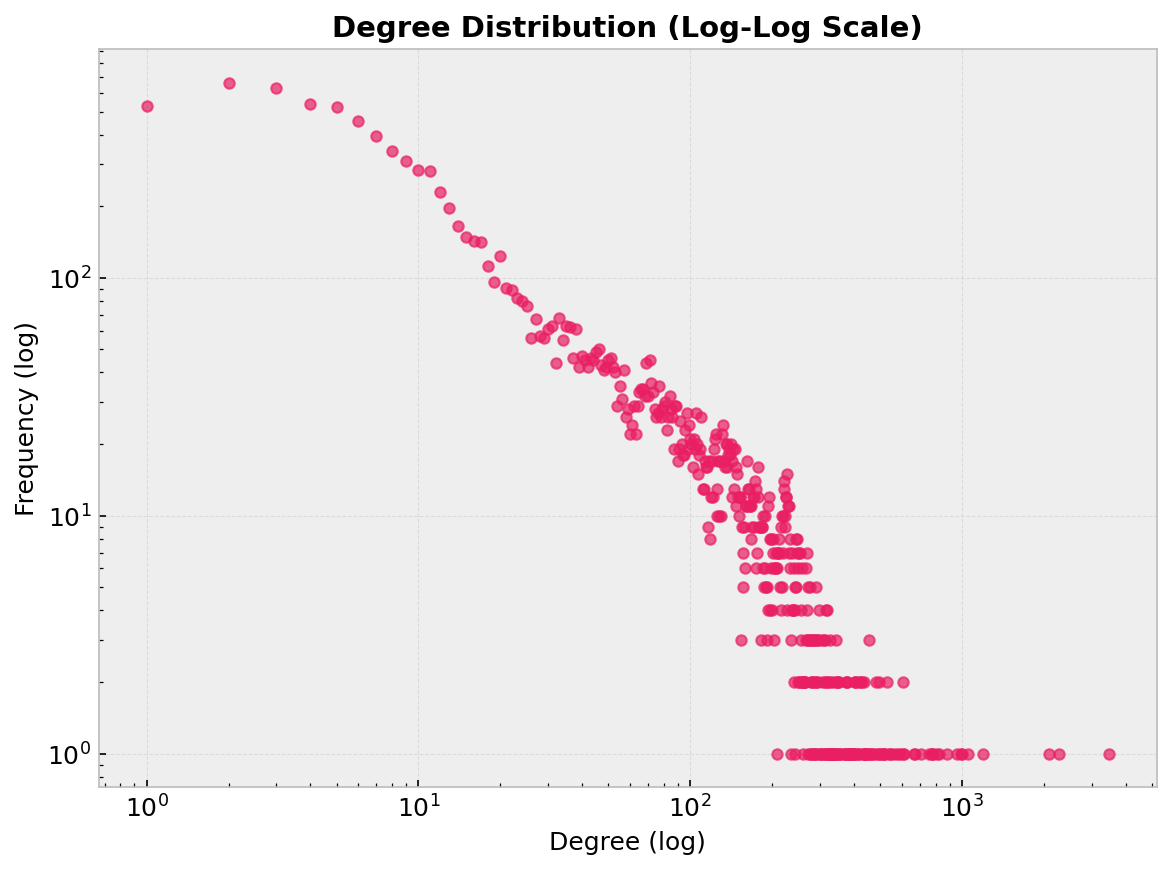
\includegraphics[width=0.78\textwidth]{figures/degree-log-log.png}
\caption{Distribution degre-degre en echelle log-log du graphe Custom-WikiCS nettoye.}
\label{fig:final-degree-loglog}
\end{figure}

Le comportement ajuste par loi de puissance a motive les experiences de
correction sensibles au degre, ensuite utilisees dans les modeles structurels
et hybrides. Le graphe est egalement assortatif sur le plan semantique: les
paires d'articles liees sont plus semblables que des paires aleatoires dans
l'espace des embeddings.

\begin{figure}[H]
\centering
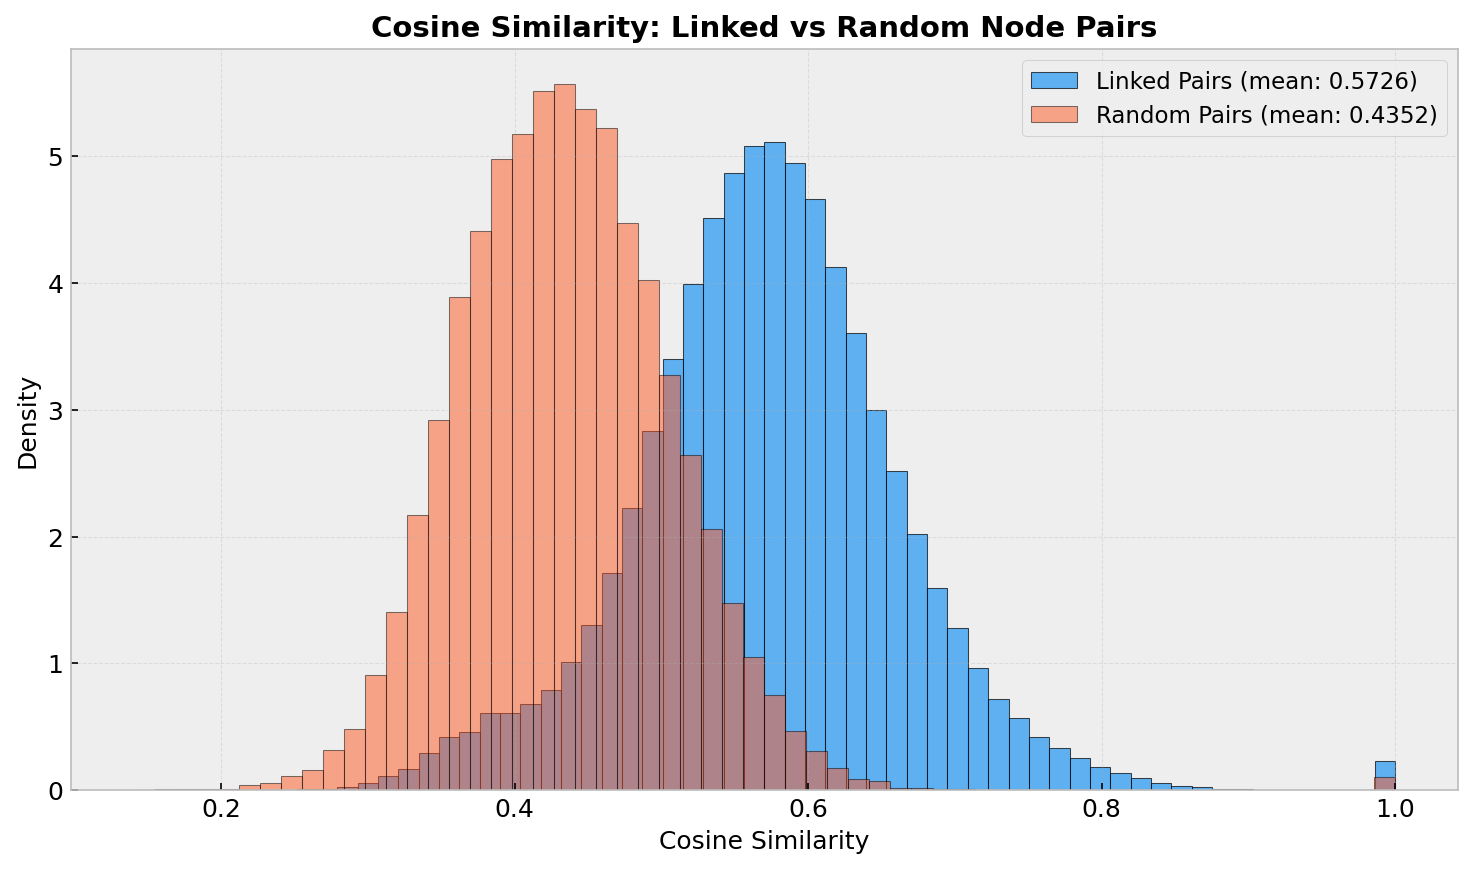
\includegraphics[width=0.82\textwidth]{figures/cosine-similarity-assortativity.png}
\caption{Distributions de similarite cosinus pour des paires d'articles liees par rapport a des paires aleatoires.}
\label{fig:final-cosine-assort}
\end{figure}

Enfin, l'analyse de centralite et de communautes montre que le graphe n'est ni
plat ni uniformement melange. Cela importe pour la recommandation, car les
effets de popularite, la domination des hubs et les communautes locales
influencent tous les articles qu'un modele a tendance a faire remonter.

\begin{figure}[H]
\centering
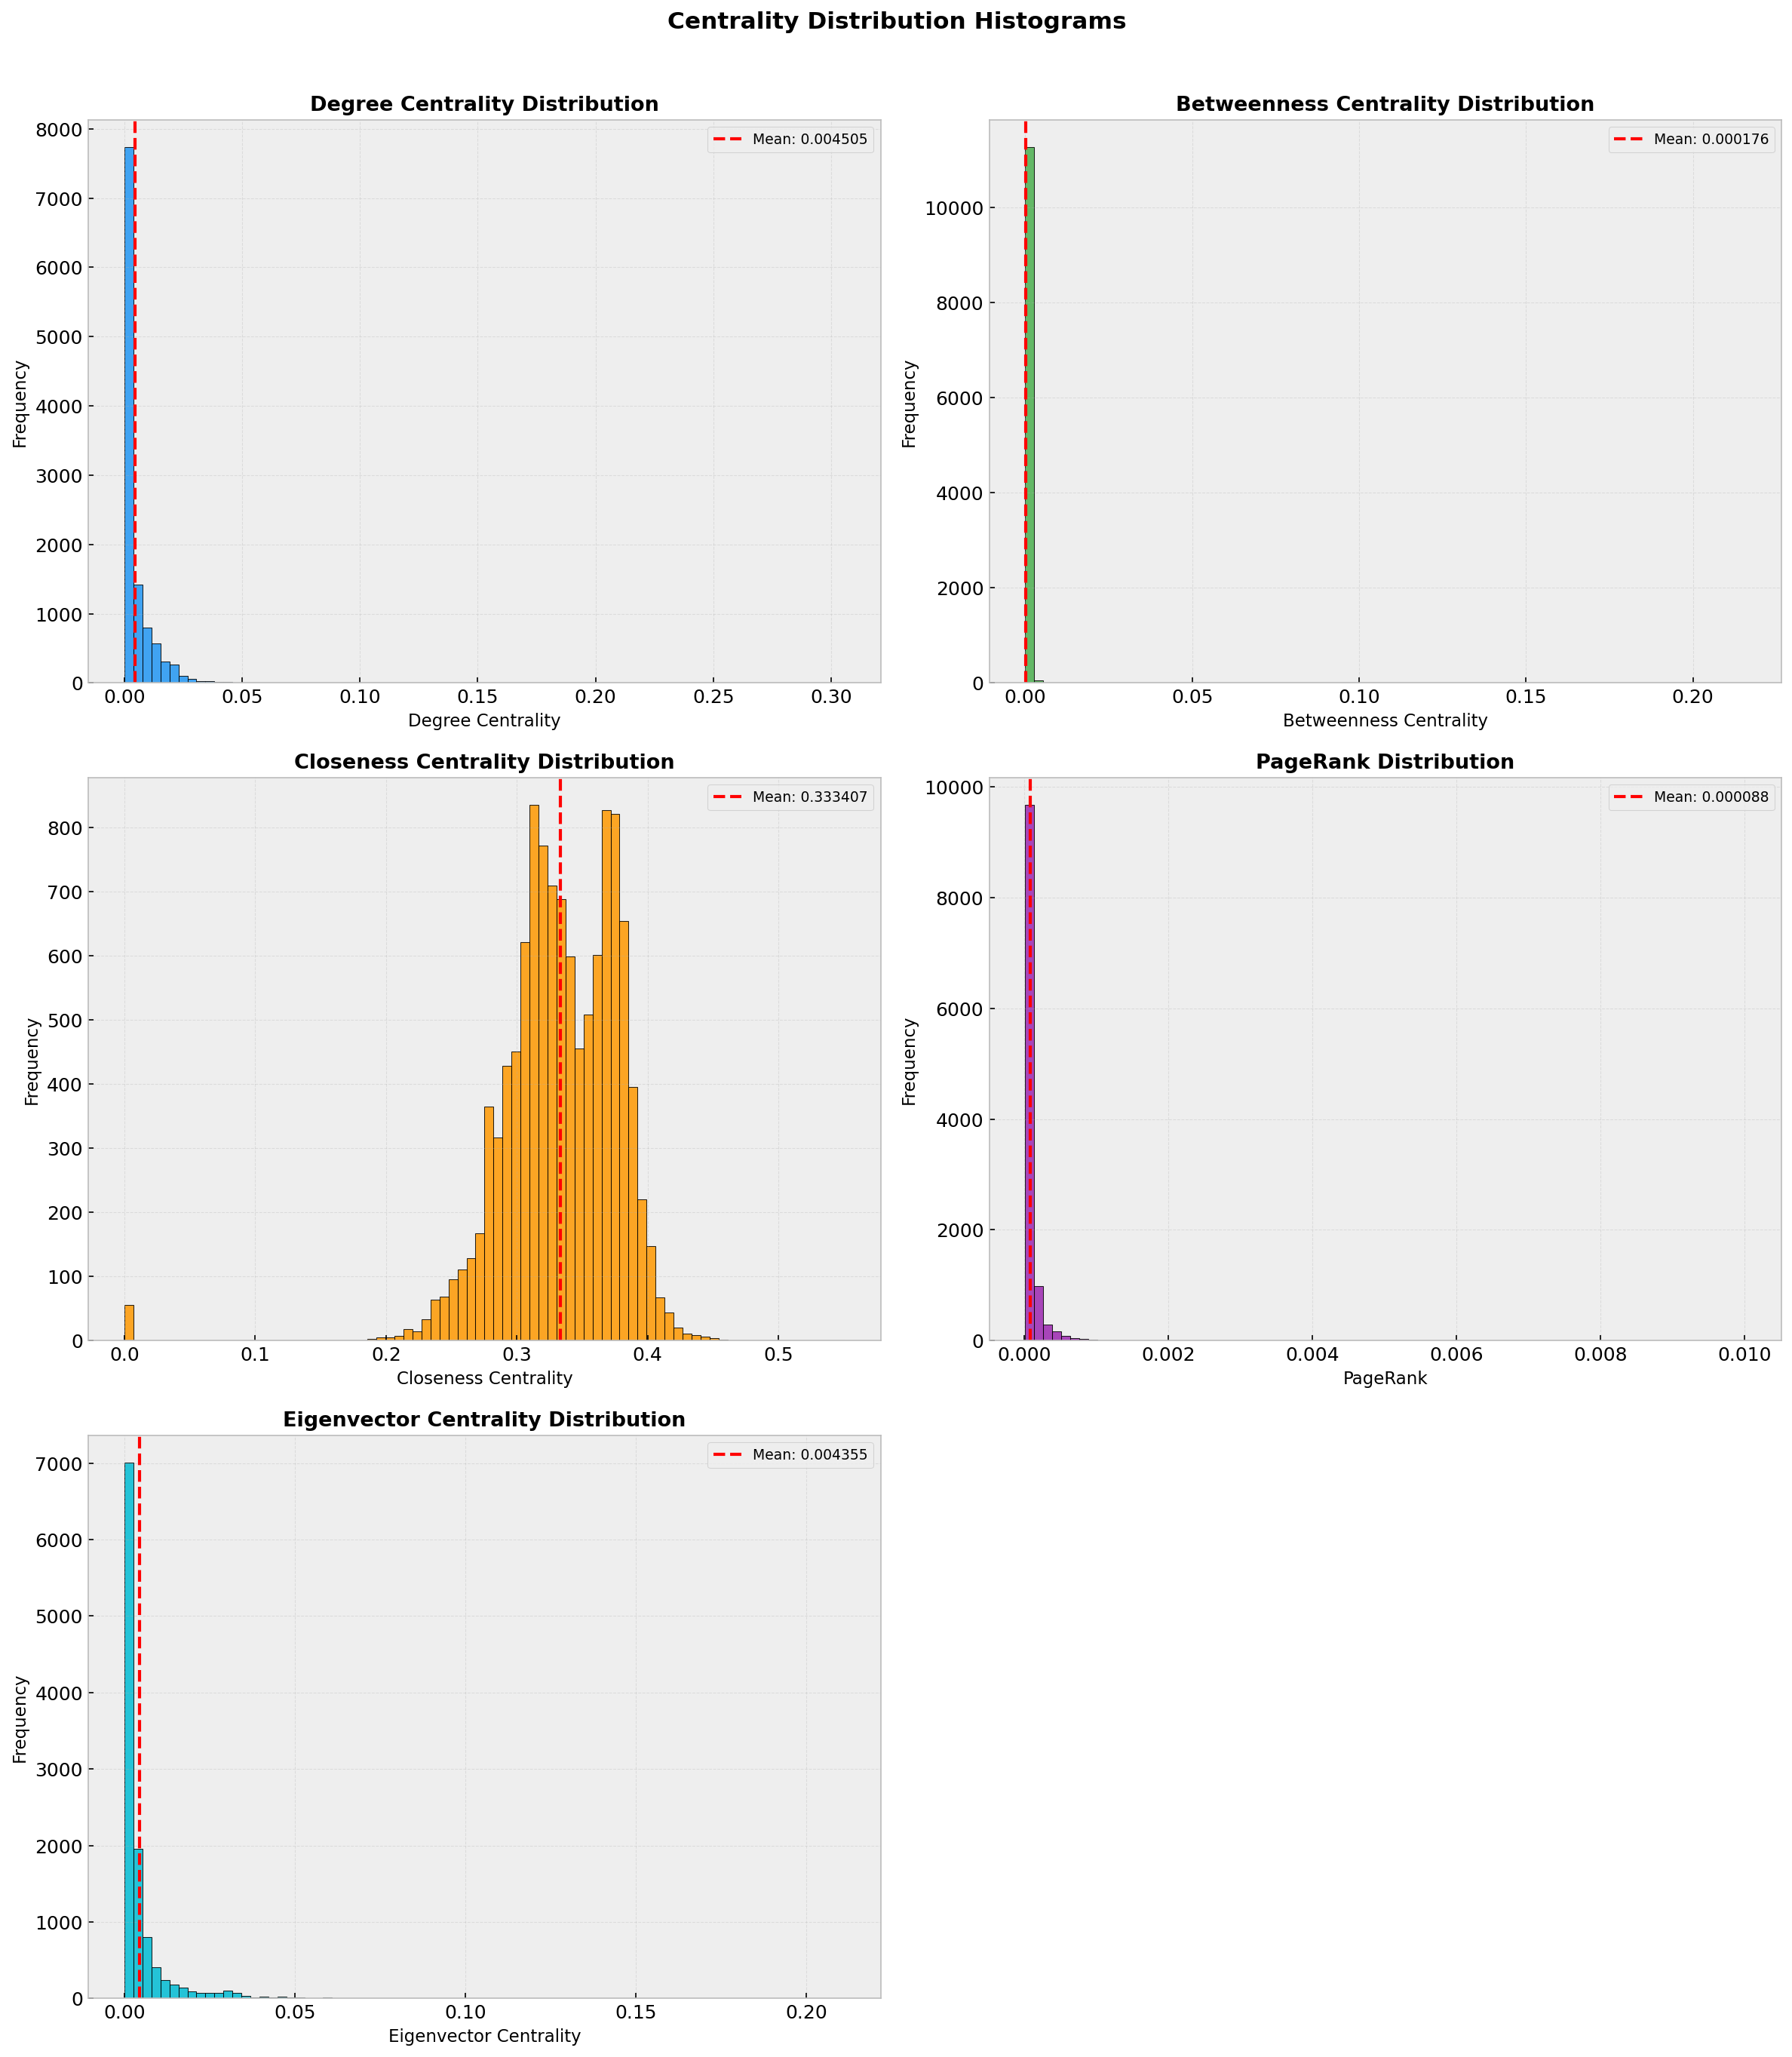
\includegraphics[width=0.86\textwidth]{figures/centrality-histograms.png}
\caption{Distributions de centralite dans le graphe d'articles nettoye.}
\label{fig:final-centrality}
\end{figure}

\begin{figure}[H]
\centering
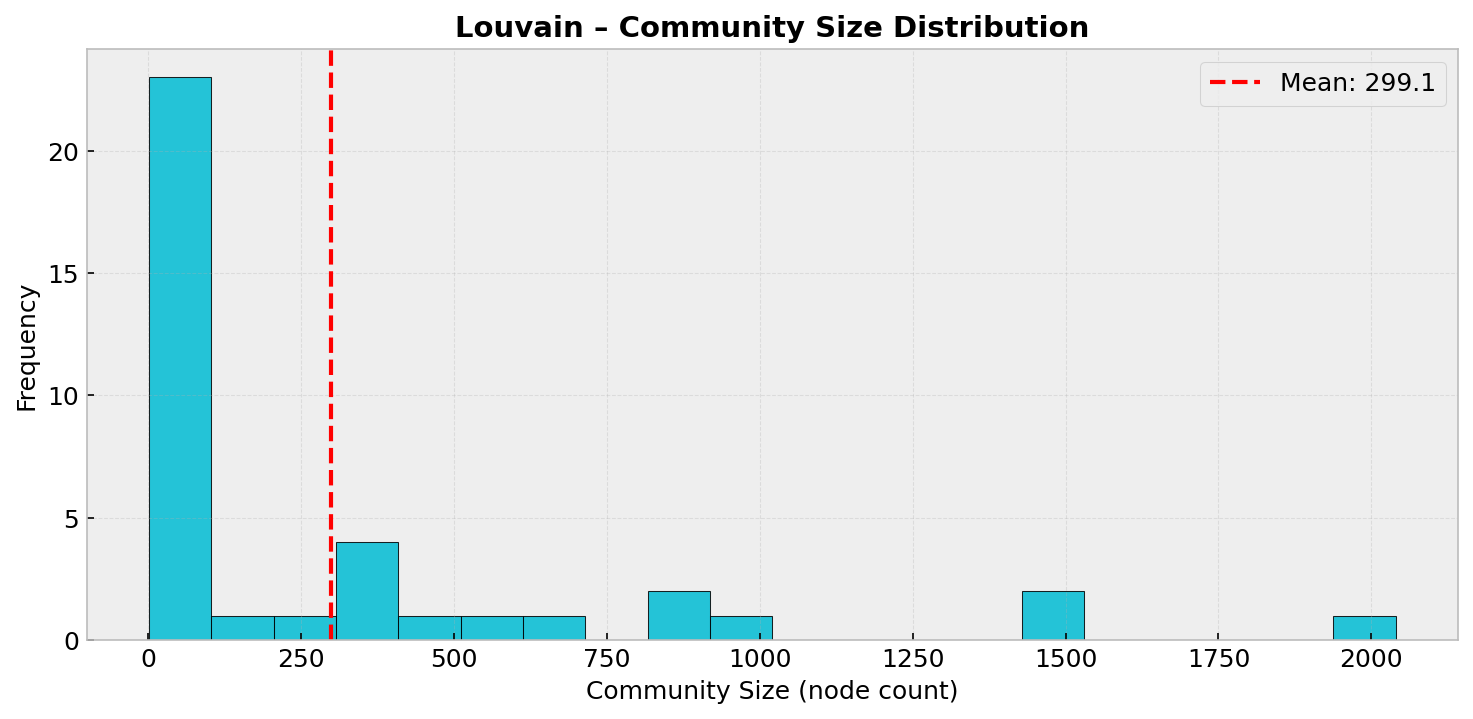
\includegraphics[width=0.82\textwidth]{figures/community-size-distribution-louvain.png}
\caption{Distribution des tailles de communautes Louvain dans le graphe nettoye.}
\label{fig:final-louvain}
\end{figure}

\section{Resultats de l'evaluation initiale}

Le premier pipeline complet de recommandation combinait BGE-M3 avec une
representation structurelle derivee de Node2Vec et evaluait le resultat sur des
aretes mises de cote. Cette premiere evaluation rapportait:
\begin{itemize}
    \item Hit@10 = 11.49\%,
    \item MRR = 0.0548.
\end{itemize}

L'étape majeure suivante a consisté en la comparaison de huit modèles, résumée dans les comparaisons initiales. 
Dans ce premier dispositif d'evaluation, Node2Vec non corrige
semblait dominer la famille de modeles.
Le Tableau~\ref{tab:final-report6-topline} reproduit les resultats les plus
importants des comparaisons initiales, car ils fournissent le recit de reference qui a du etre
reexamine par la suite.

\begin{table}[H]
\centering
\caption{Principaux resultats de l'ancienne evaluation a huit modeles.}
\label{tab:final-report6-topline}
\begin{tabular}{lcc}
\toprule
\textbf{Modele} & \textbf{Hit@10} & \textbf{MRR} \\
\midrule
Node2Vec (uncorrected) & 16.06\% & 0.0751 \\
GCN + BGE-M3 (rank fusion) & 11.04\% & 0.0495 \\
BGE-M3 Only & 10.20\% & 0.0506 \\
BGE-M3 + Node2Vec (corrected) & 9.82\% & 0.0471 \\
GCN Only & 6.20\% & 0.0302 \\
GraphSAGE Only & 1.43\% & 0.0087 \\
\bottomrule
\end{tabular}
\end{table}

\section{Resultats de l'evaluation revisee}

La principale contribution numerique de la phase ulterieure est un protocole
revise d'evaluation structurelle non orientee. Dans ce cadre, le projet
compare dix modeles et ajoute une seconde famille de metriques de qualite de
recommandation. Le Tableau~\ref{tab:final-combined-metrics} donne la table
complete des resultats revises.

\begin{table}[H]
\centering
\caption{Metriques combinees de classement et de qualite de recommandation sous l'evaluation revisee.}
\label{tab:final-combined-metrics}
\setlength{\tabcolsep}{3pt}
\renewcommand{\arraystretch}{1.12}
\resizebox{\textwidth}{!}{
\begin{tabular}{@{}l*{13}{c}@{}}
\toprule
\textbf{Modele} &
\textbf{H@1} &
\textbf{H@10} &
\textbf{H@50} &
\textbf{H@100} &
\textbf{MRR} &
\textbf{NDCG} &
\textbf{Recall} &
\textbf{MAP} &
\textbf{Pop. Lift} &
\textbf{Gini} &
\textbf{Agg. Div.} &
\textbf{Novelty} &
\textbf{ILD} \\
\midrule
BGE pooled + Node2Vec (corrected) & 1.03\% & 8.67\% & 31.46\% & 47.81\% & 0.0410 & 0.1160 & 0.4781 & 0.0392 & 1.3301 & 0.4110 & 11,326 & 14.2738 & 0.4372 \\
BGE-M3 + Node2Vec (corrected) & 1.07\% & 8.67\% & 32.41\% & 49.81\% & 0.0421 & 0.1202 & 0.4981 & 0.0403 & 1.3081 & 0.4127 & 11,268 & 14.2783 & 0.4316 \\
BGE pooled + Node2Vec (uncorrected) & 0.76\% & 7.83\% & 32.64\% & 50.74\% & 0.0376 & 0.1176 & 0.5074 & 0.0358 & 1.3397 & 0.4613 & 11,186 & 14.0351 & 0.4558 \\
BGE-M3 + Node2Vec (uncorrected) & 0.76\% & 7.83\% & 32.64\% & 50.74\% & 0.0376 & 0.1176 & 0.5074 & 0.0358 & 1.3400 & 0.4605 & 11,164 & 14.0340 & 0.4557 \\
Node2Vec (uncorrected) & 0.75\% & 7.81\% & 32.52\% & 50.60\% & 0.0375 & 0.1172 & 0.5060 & 0.0357 & 1.3374 & 0.4482 & 10,966 & 14.0466 & 0.4569 \\
Node2Vec (corrected) & 0.75\% & 7.81\% & 32.52\% & 50.60\% & 0.0375 & 0.1172 & 0.5060 & 0.0356 & 1.3374 & 0.4482 & 10,966 & 14.0466 & 0.4569 \\
GCN + BGE-M3 (rank fusion) & 0.85\% & 7.63\% & 23.14\% & 33.77\% & 0.0335 & 0.0862 & 0.3377 & 0.0317 & 1.6650 & 0.4228 & 11,655 & 13.9222 & 0.4366 \\
BGE-M3 Only & 1.35\% & 7.57\% & 19.69\% & 27.73\% & 0.0366 & 0.0788 & 0.2773 & 0.0351 & 1.9413 & 0.5172 & 10,905 & 13.8459 & 0.3713 \\
GCN Only & 0.38\% & 3.46\% & 14.12\% & 22.91\% & 0.0180 & 0.0530 & 0.2291 & 0.0163 & 1.1879 & 0.2607 & 11,685 & 14.3293 & 0.5135 \\
GraphSAGE Only & 0.17\% & 1.22\% & 4.96\% & 8.72\% & 0.0076 & 0.0199 & 0.0872 & 0.0061 & 1.3134 & 0.2517 & 11,628 & 14.2087 & 0.5313 \\
\bottomrule
\end{tabular}
}
\end{table}

\section{Extension de metriques}

La ligne de rapports ulterieure a ajoute une couche de mesure a seuil plus
court et centree sur l'AUC, sans modifier le cadre d'evaluation sous-jacent.
Le Tableau~\ref{tab:final-eval31-metrics} reproduit les metriques de
l'extension.

\begin{table}[H]
\centering
\caption{Metriques de l'extension sous l'evaluation revisee.}
\label{tab:final-eval31-metrics}
\setlength{\tabcolsep}{4pt}
\renewcommand{\arraystretch}{1.12}
\resizebox{\textwidth}{!}{
\begin{tabular}{@{}l*{6}{c}@{}}
\toprule
\textbf{Modele} &
\textbf{H@10} &
\textbf{NDCG@10} &
\textbf{Recall@10} &
\textbf{MAP@10} &
\textbf{ROC-AUC} &
\textbf{PR-AUC} \\
\midrule
BGE pooled + Node2Vec (corrected) & 8.67\% & 0.0409 & 8.67\% & 0.0273 & 0.9563 & 0.9559 \\
BGE-M3 + Node2Vec (corrected) & 8.67\% & 0.0413 & 8.67\% & 0.0278 & 0.9582 & 0.9579 \\
BGE pooled + Node2Vec (uncorrected) & 7.83\% & 0.0356 & 7.83\% & 0.0229 & 0.9710 & 0.9716 \\
BGE-M3 + Node2Vec (uncorrected) & 7.83\% & 0.0356 & 7.83\% & 0.0229 & 0.9710 & 0.9716 \\
Node2Vec (uncorrected) & 7.81\% & 0.0355 & 7.81\% & 0.0229 & 0.9717 & 0.9714 \\
Node2Vec (corrected) & 7.81\% & 0.0355 & 7.81\% & 0.0228 & 0.9717 & 0.9714 \\
BGE-M3 Only & 7.64\% & 0.0406 & 7.64\% & 0.0298 & 0.8851 & 0.8886 \\
GCN + BGE-M3 (rank fusion) & 7.63\% & 0.0355 & 7.63\% & 0.0234 & 0.9356 & 0.9363 \\
GCN Only & 3.46\% & 0.0161 & 3.46\% & 0.0107 & 0.8954 & 0.8946 \\
GraphSAGE Only & 1.22\% & 0.0060 & 1.22\% & 0.0041 & 0.8691 & 0.8561 \\
\bottomrule
\end{tabular}
}
\end{table}

Ces tableaux constituent la base quantitative de l'interpretation discutee dans
le chapitre suivant.
